\documentclass[
reprint,amsmath,amssymb,aps]{revtex4-2}

\usepackage{graphicx}
\usepackage{dcolumn}
\usepackage{bm}
\usepackage{float}
\usepackage{tabularx}
\usepackage{multirow}
\usepackage{braket}
\usepackage{amsmath}


\begin{document}

\preprint{APS/123-QED}

\title{Spin dynamics and magnetic bistability in single Dy adatoms on graphene/Ir(111)
studied by SP-STM}

\author{A. Curcella}
 \email{Equally contributed to this work} 
\affiliation{Institute of Physics, Ecole Polytechnique Fédérale de Lausanne, CH-1015 Lausanne, Switzerland}

\author{D. Sblendorio}
 \email{equally contributed to this workw}
\affiliation{Institute of Physics, Ecole Polytechnique Fédérale de Lausanne, CH-1015 Lausanne, Switzerland}

\author{S. Rusponi}
\affiliation{Institute of Physics, Ecole Polytechnique Fédérale de Lausanne, CH-1015 Lausanne, Switzerland}

\author{M. Pivetta}
\affiliation{Institute of Physics, Ecole Polytechnique Fédérale de Lausanne, CH-1015 Lausanne, Switzerland}

\author{F. Patthey}
\affiliation{Institute of Physics, Ecole Polytechnique Fédérale de Lausanne, CH-1015 Lausanne, Switzerland}

\author{H. Brune}
\affiliation{Institute of Physics, Ecole Polytechnique Fédérale de Lausanne, CH-1015 Lausanne, Switzerland}
 

\begin{abstract}
The magnetic stability in single Dy adatoms on graphene/Ir(111) is investigated by means of spin-polarized scanning tunneling microscopy at liquid He temperature. Telegraph-noise traces demonstrate the bistability of the Dy magnetization, and exhibit long relaxation times of several minutes, consistent with previous XMCD measurements \citep{baltic2016}.
The asymmetric occupancy of the magnetic states as a function of tunnel voltage is evidence for a spin-torque exerted by tunneling electrons on the single-atom magnet \citep{Khajetoorians2013,delgado2010}.
Based on existing theoretical works, we implement a model that quantitatively reproduces the asymmetry in the occupancy of the magnetic states and their average lifetimes, the temperature dependence of the magnetization reversal, and the value of the magnetoresistive contribution in the STM current. 
\end{abstract}

\maketitle

\section{Introduction}
Manipulation of the magnetic states of nano-objects and in surface adsorbed single adatoms offer novel avenues for exploring the fundamental physics that determine their behavior. Understanding this behavior is essential for the development of future spintronic devices and the realization of ultra-high-density magnetic memory [citations...]. The injection of a spin-polarized current can efficiently reorient the magnetization of a nanomagnet \citep{Khajetoorians2013,krause_joule_2011,loth2010}, enabling the possibility of reading and writing of the magnetic states.
Dysprosium atoms adsorbed on a single graphene layer grown on Ir(111) were identified as stable single-atom magnets \citep{baltic2016}. Previous scanning tunneling microscopy (STM) studies revealed these atoms self assemble into a highly-ordered superlattice after annealing at 40~K \citep{baltic2016,pivetta2018}. Obtaining uniformly dispersed bi-stable magnetic nanostructures on a decoupling atomic layer is a paramount achievement for the development of ultra-high magnetic memory densities [citations]. Previous x-ray magnetic circular dichroism (XMCD) measurements revealed that Dy adatoms on graphene/Ir(111) possess a \textit{4f$^{\:10}$} occupation, a \textit{J} = 8 total angular momentum identical to Dy in the gas phase, and a \textit{J$_z$} = $\pm$7 out-of-plane magnetic ground state \citep{baltic2016,baltic2018}.
The measured spin lifetimes are of the order of 1000~s at 2.5~K.
However, the lifetimes obtained by XMCD are limited by the interaction of the adatoms with photon-induced secondary electrons. The extrapolation of the intrinsic magnetization lifetime at zero photon flux represents a lower bound estimate.

Here we present the results of a SP-STM study conducted on well-isolated Dy adatoms adsorbed on Gr/Ir(111). We implement a model which accounts for the recently observed intra-atomic interaction between internal \textit{4f} and external \textit{6s-5d} polarized shells \cite{pivetta2020}, offering an original revision of the description of the spin-dynamics in rare-earth based single-adatom magnets. The Dy adatoms adsorb onto the sixfold graphene hollow site \cite{baltic2018}. The crystal field lifts the degeneracy of the magnetic states and gives rise to a strong out-of-plane easy-axis anisotropy.
If the intra-atomic exchange is neglected, \textit{i.e.} the external shells are not polarized, the magnetic states $\ket{M}$ are defined solely by the magnetic moment of the \textit{4f} shell $\ket{M}=\ket{j_{4f}}$, Fig.~\ref{fig:intra}a. The term $B_6^6$ in the crystal field (see Supplemental) mixes the states with $\Delta j_{4f}=6n$, with $n\in \mathbb{Z}$. 
Fig.~\ref{fig:intra}b represents the zero-field level scheme diagram when no intra-atomic exchange is considered. The red-shaded areas represent the mixing and the zero-field splitting $\omega$ of the states $\ket{j_{4f}}=\ket{\pm 6}$ and $\ket{j_{4f}}=\ket{\pm 3}$. However, once the intra-atomic exchange coupling is included in the Hamiltonian, \textit{i.e.} the external shells are polarized, the new basis now includes the magnetic moment of the internal \textit{4f} shell, and of the external \textit{5d} and \textit{6s} ones: $\ket{M}=\ket{m_i}=\ket{j_{4f},s_{5d},s_{6s}}$, as shown in Fig.~\ref{fig:intra}d.
In this new basis, the $B_6^6$ term of the crystal field mixes the states with $\Delta M_{tot}=\Delta j_{4f} + \Delta s_{5d} + \Delta s_{6s}=6n$, with $n\in \mathbb{N}$. This results in the mixing and splitting of the states $\ket{M}=\ket{m_{\pm 5}}$ and $\ket{M}=\ket{m_{\pm 8}}$, see Fig.~\ref{fig:intra}e, which have $\Delta M_{tot}\sim 12$ and $\Delta M_{tot}\sim 18$, respectively. The intra-atomic exchange keeps the magnetic moment in the external and internal shells aligned \cite{pivetta2020}, as it can be seen in Fig.~\ref{fig:intra}f. The mixing of states determine the preferential pathways through which the magnetization can tunnel through the anisotropy barrier. Thus, the pathways for the magnetization reversal are unique to the choice of basis. 
\begin{figure*}[ht!]
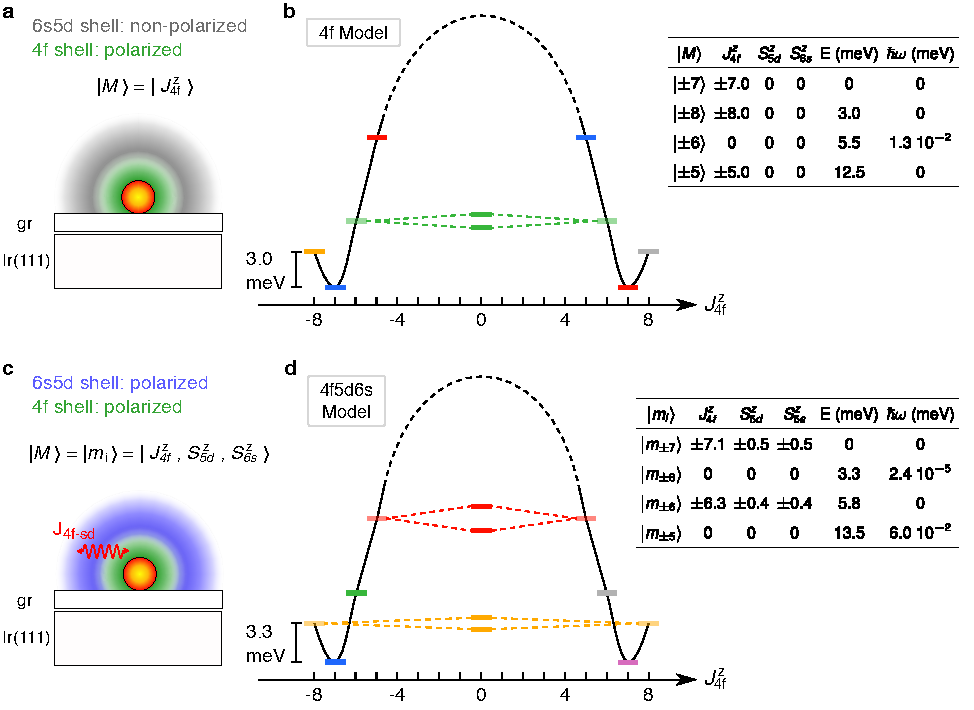
\includegraphics[width=0.98\textwidth]{Fig1_new.pdf}
\caption{Intra-atomic vs no intra-atomic
\label{fig:intra} }
\end{figure*}
Furthermore, we describe the mechanisms by which the magnetization is driven out of the ground states $\ket{M}=\ket{\pm7}$ and into the higher energy states that allow for magnetization reversal to occur. Without the influence of the tip (Fig.~\ref{fig:no_tip_tip_telegraph}a) only substrate electrons and phonons can drive the magnetization out of equilibrium. Phonons can be interpreted as a deformation of the substrate, perturbing the crystal field \citep{cervetti2016}, and influencing the external $4f$-shell due to its non-vanishing orbital component (see supplemental for the Hamiltonian term). Phonons can induce transitions with $\Delta m = \pm 1$, and $\Delta m = \pm 2$ \citep{cervetti2016}. We assume that the spins grafted on graphene experience the effect of a two-dimensional phonon bath \citep{cervetti2016}. The transition rates between the states $\ket{M}$ and $\ket{M^{\prime}}$ write:

\begin{equation}
    \label{eq:phonon_rates}
    W_{M,M^{\prime}}^{ph}=\dfrac{3 \nu_{ph}}{2\theta_{Dy}\rho_{gr}c_{gr}^4 \hbar^3} \mathcal{P} \left( \Delta E_{M,M^{\prime}}, T \right) w^{ph}_{M,M^{\prime}}
\end{equation}

in which $\nu_{ph}$ is the only unknown parameter and it represents the phonon-spin coupling cross section, $c_{gr}$ is the speed of sound in graphene, $\rho_{gr}$ is the graphene density, $\theta_{Dy}$ is the Dy coverage referred to a graphene monolayer. $\mathcal{P}\left( \Delta E_{M,M^{\prime}}, T \right)$ depends on the Bose-Einstein distribution at the sample temperature $T$ and on $\Delta E_{M,M^{\prime}}$, \textit{i.e.} the energy difference between the states $\ket{M}$ and $\ket{M^{\prime}}$. $w^{ph}_{M,M^{\prime}}$ are the phonon matrix elements, for which we assume that phonons act only on the external $4f$ shell (see Supplemental).
% \begin{align}
%     \label{eq:ph_abs}
%     W_{M,M^{\prime}}^{ph} & =\dfrac{3 \nu_{ph}\Delta E_{M,M^{\prime}}^2}{2\theta_{Dy}\rho_{gr}c_{gr}^4 \hbar^3}\dfrac{1}{e^{\Delta E_{M,M^{\prime}}\beta}-1}w^{ph}_{M,M^{\prime}}\\
%     W_{M,M^{\prime}}^{ph} & =\dfrac{3 \nu_{ph} \Delta E_{M,M^{\prime}}^2}{2\theta_{Dy}\rho_{gr}c_{gr}^4 \hbar^3}\left(\dfrac{e^{\Delta E_{M,M^{\prime}}\beta}}{e^{\Delta E_{M,M^{\prime}}\beta}-1}\right)w^{ph}_{M,M^{\prime}}
%     \label{eq:ph_emis}
% \end{align}

%for the adsorption and emission of a phonon, respectively. In the equations, $\nu_{ph}$ is the only unknown parameter and it represents the phonon-spin coupling cross section, $c_{gr}$ is the speed of sound in graphene, $\rho_{gr}$ is the graphene density, $\theta_{Dy}$ is the Dy coverage referred to a graphene monolayer, $\beta=1/k_bT$ and $T$ is the sample temperature. $\Delta E_{M,M^{\prime}}$ represents the energy difference between the states $\ket{M}$ and $\ket{M^{\prime}}$, and it is equal to the zero-field splitting $\omega$ when there is no external magnetic field. $w^{ph}_{M,M^{\prime}}$ are the matrix elements, they are calculated assuming that phonons act only on the external $4f$ shell (see Supplemental).
The other contribution limiting the spin-lifetime of the Dy adatoms is the scattering with the substrate electrons, represented by $e^{-}_{SS}$ in Fig.\ref{fig:no_tip_tip_telegraph}a. The creation or annihilation of an electron hole pair in the substrate induces a spin transition ($\Delta m=\pm 1$) in the external \textit{6s-5d} shell \cite{}"loth paper about tunneling through ext shells". Consequently, the magnetic moment of the $4f$ shell flips, because the intra-atomic exchange interaction forces the magnetization alignment of the coupled internal and external shells \cite{pivetta2020}. We consider a non-polarized substrate, so that substrate electrons scattering bolsters an equal occupation of the doubly degenerate ground state.\newline
\indent We can now expand the model to describe SP-STM experimental conditions.
\begin{figure*}[ht!]
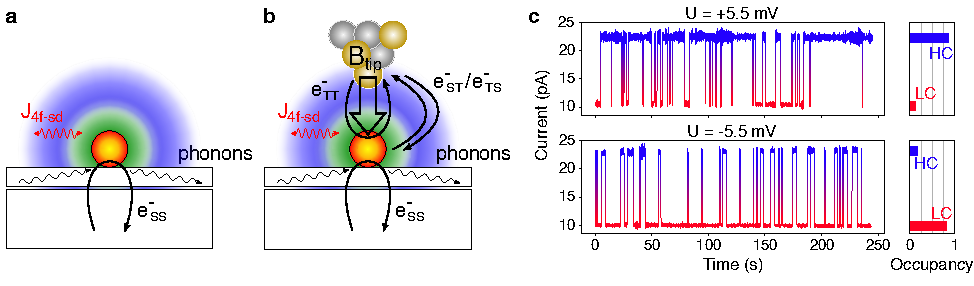
\includegraphics[width=0.98\textwidth]{Fig2_new.pdf}
\caption{Intra-atomic vs no intra-atomic
\label{fig:no_tip_tip_telegraph} }
\end{figure*}
%, as sketched in Fig.~\ref{fig:no_tip_tip_telegraph}b. 
In SP-STM experiments, we use an anti-ferromagnetic MnNi tip to measure the magnetization state of an isolated Dy adatom via magnetoresistive effect \cite{}. The fixed spin-polarization of the tip enables the measurement of the spin-lifetimes of the ground-states $\ket{m_{\pm7}}$, the spin-lifetimes of the excited states being too short to be detected within the bandwidth of available current-sensing electronics. Fig.~\ref{fig:no_tip_tip_telegraph}c shows two telegraph-noise signal traces in which the tunneling current switches between a high-conductance (HC) and low-conductance (LC) state, corresponding to matching or opposite spin-polarization of the tip and of the adatom ground-state, respectively \cite{}. 
%brief description of the experiments
The mechanisms determining the spin-lifetimes of Dy in SP-STM measurements are sketched in Fig.~\ref{fig:no_tip_tip_telegraph}b.
Firstly, the magnetic tip generates a magnetic field having a dipolar $B_{dip}$ and an exchange $B_{ex}$ contribution. The relative strength of the two components depends on the tip-adatom distance $d_{TS}$ \cite{willke}. 
The tip field is defined by the dipolar $B^0_{dip}$ and exchange $B^0_{ex}$ component at a tip-sample distance of $d_{TS}=5$ \AA (see supplemental). The dipolar field scales with $1/d_{TS}^3$ and acts on all the polarized shell. For simplicity, we consider the exchange contribution to have a pure exponential dependence on tip-sample distance, $\propto e^{-d_{TS}/\lambda_{ex}}$, where $\lambda_{ex}$ is the exchange decay length \cite{}.
As the exchange interaction is a function of the superposition between the tip and adatom electronic wavefunctions, we assume that the exchange tip field component acts only on the external \textit{6s-5d} shell.
The tip field shifts the magnetic states via Zeeman interaction, which acts on the polarized shells proportionally to their magnetic moment and an effective g-factor (see Supplemental). 
The ground states $\ket{m_{\pm7}}$  are shifted apart in energy, lifting the degeneracy. In second place, we consider the scattering with tip electrons, $e^{-}_{TT}$ in Fig.~\ref{fig:no_tip_tip_telegraph}a. An electron originating in the tip can transfer its energy and momentum to an external Dy electron ($\Delta m=\pm 1$), eventually tunneling back to the tip. The magnetic tip used in SP-STM experiments is characterized by a spin-up $\rho_{T\uparrow}$ and spin-down $\rho_{T\downarrow}$ populations at the Fermi level. The asymmetry in the population engenders a higher probability of spin-increasing ($\Delta m=+1$) or spin-decreasing ($\Delta m=-1$) transitions in the Dy adatom. Note that neither $e^{-}_{SS}$ nor $e^{-}_{TT}$ electrons contribute to the tunneling current, but they do affect the spin dynamics of the system. Finally, we consider the tunneling electrons, $e^{-}_{TS}$ and $e^{-}_{ST}$ in Fig.~\ref{fig:no_tip_tip_telegraph}b. The fraction of these electrons that do not exchange their momentum with the Dy adatom, constitute the elastic contribution to the current, while those inducing spin transitions builds up the inelastic part. The proportion between spin-increasing and spin-decreasing transitions induced by the inelastic current reflects the tip spin-polarization. Formally, the coupling between adatom and electrodes, \textit{i.e.} the tip and the substrate, is modeled by a Kondo-type Hamiltonian \cite{delgado2010} (see Supplemental). The transition rates associated with sample-to-sample ($e^{-}_{SS}$), tip-to-tip ($e^{-}_{TT}$), tip-to-sample ($e^{-}_{TS}$) and sample-to-tip ($e^{-}_{ST}$) can be compactly written as:
% \begin{equation}
%  \begin{split}
%     W_{M,M^{\prime}}^{\eta}=\sum_{a=+,-,z} w_{M,M^{\prime}}^a \dfrac{2\pi}{\hbar} \zeta^2 \left( &\varsigma_{\eta}\varsigma_{\eta^{\prime}} Q_{\eta \eta^{\prime}}^a \mathcal{F}_{\eta \eta^{\prime}}(\Delta E_{M,M^{\prime}},U)\\
%      & +\varsigma_{\eta}^2  Q_{\eta \eta}^a  \mathcal{F}_{\eta \eta}(\Delta E_{M,M^{\prime}}) \right)
%  \end{split}
% \end{equation}

\begin{equation}
    W_{M,M^{\prime}}^{\eta}=\dfrac{2\pi}{\hbar} \zeta^2 \varsigma_{\eta} \left( K_{\eta \eta^{\prime}}+ K_{\eta \eta} \right)w_{M,M^{\prime}}^{el}, \qquad \eta,\eta^{\prime}=T,S
    \label{eq:elec_rates}
\end{equation}

in which $w_{M,M^{\prime}}^{el}$ are the matrix elements describing the interaction with the external $6s-5d$ electrons, $\varsigma_{\eta}$ is the coupling with the electrode $\eta$, $\zeta$ is the ratio between inelastic and elastic tunneling matrix elements, that for simplicity we assume to be the same for tip and sample. $K_{\eta \eta^{\prime}}$ accounts for the scattering from the actual tunneling electrons ($e^{-}_{TS}$, $e^{-}_{ST}$) , while $K_{\eta \eta}$ is the analogous for the electrons originating and ending in the same electrode ($e^{-}_{SS}$, $e^{-}_{TT}$) and they are defined as:
\begin{align}
    &K_{\eta \eta^{\prime}}=\varsigma_{\eta^{\prime}} \rho_{\eta \eta^{\prime}}\mathcal{F}_{\eta \eta^{\prime}}(\Delta E_{M,M^{\prime}},U,T) \\
    &K_{\eta \eta}=\varsigma_{\eta} \rho_{\eta \eta}\mathcal{F}_{\eta \eta}(\Delta E_{M,M^{\prime}},0,T) 
\end{align}

in which $\rho_{\eta \eta^{\prime}}$ and $\rho_{\eta \eta}$ are the convoluted spin-dependent populations, while $\mathcal{F}_{\eta \eta^{\prime}}(\Delta E_{M,M^{\prime}},U,T)$ and $\mathcal{F}_{\eta \eta}(\Delta E_{M,M^{\prime}},0,T)$ include the Fermi distribution of the electrons at temperature $T$, and they depend on the bias voltage between tip and sample $U$ (vanishing for $e^{-}_{SS}$ and $e^{-}_{TT}$ electrons) and on the energy separation $\Delta E_{M,M^{\prime}}$ between the states involved in the transition.

%To determine the contributions of the previous mechanisms acting in the spin dynamics of Dy/Gr/Ir(111), we have determined spin-lifetimes and occupancy from telegraph-noise traces measured as a function of bias $U$, temperature $T$, and current $I_{set}$. 

We employ the model just presented to reproduce the spin-lifetimes and the occupancy extrapolated from telegraph-noise traces, similar to those in Fig. \ref{fig:no_tip_tip_telegraph}c, that we measuer as a function of bias $U$, temperature $T$, and current $I_{set}$. The calculated values are obtained by solving the following master equations, using the transition rates in Eqs.~\ref{eq:phonon_rates} and \ref{eq:elec_rates}:
\begin{align}
%\dfrac{dP_M}{dt}= & -P_M \sum_{M\neq M^{\prime}}\left[ \left(  W_{M,M^{\prime}}^{\eta} \right) +P_{M^{\prime}}\left(  W_{M^{\prime},M}^{\eta} \right) \right] + Q_M^{QTM} \left(P_{-M}- P_{M} \right)
\begin{split}
\dfrac{dP_M}{dt}=&-P_M \sum_{M\neq M^{\prime}}\left(   W_{M,M^{\prime}}^{tot}  +P_{M^{\prime}}  W_{M^{\prime},M}^{tot}  \right) \\
%&+ Q_M \left(P_{-M}- P_{M} \right)
\end{split}
\end{align}

in which $P_M$ is the population of the state $M=\ket{m_i}$ $W_{M,M^{\prime}}^{tot}=W_{M,M^{\prime}}^{ph}+W_{M,M^{\prime}}^{T}+W_{M,M^{\prime}}^{S}$ is the sum of the phonon and electron transition rates. The inclusion of quantum tunneling rates as in Refs. [] do not affect the spin-dynamics of the system in the present case (see supplemental).
%, and $Q_M$ are transition rates associated to quantum tunneling of magnetization between states $M=\ket{m_i}$ and $-M=\ket{m_{-i}}$ \cite{} (see supplemental).
We optimize the value of the free parameters describing the tip ($B^0_{dip}$, $B^0_{ex}$, $\lambda_{ex}$), and the interaction with phonons ($\nu_{ph}$) and electrons ($\zeta$, $\varsigma_{\eta}$) to get the best agreement with experimental data.




We aim at describing the spin dynamics of Dy/Gr/Ir(111), highlightin



The ratio $\zeta$ and the coupling to the electrodes $\varsigma_T$, $\varsigma_S$ are treated as free-parameters. We assume that the coupling to the surface $\varsigma_S$ is constant and that it does not depend on the position in the Moiré pattern the adatom is sitting. The coupling to the tip $\eta_T$ scales with the set tunneling current. We define $I_0$ as the average between the high-conductance (HC) and low-conductance (LC) current, see Fig.~\ref{fig:no_tip_tip_telegraph}c. By neglecting the inelastic contribution to this current, which is orders of magnitudes lower than the elastic one, we can relate $\eta_T$ to $\eta_S$ using the experimental value of $I_0$:

\begin{equation}
   \varsigma_T= \dfrac{4 \hbar I_0}{2\pi e [f(U,T)-f(-U,T)]\varsigma_S (\rho_{S\uparrow} \rho_{T\uparrow} + \rho_{S\downarrow} \rho_{T\downarrow})}
\end{equation}

where $e$ is the electron charge and $f$ is the Fermi-Dirac distribution.

SP-STM can reveal much longer lifetimes, as shown in the case of Ho adatoms on MgO/Ag(100) \citep{Natterer2017,Natterer2018,Forrester2019}, despite the non-negligible interaction with tunneling electrons [citations].
In the present study, we investigate the spin dynamics of single Dysprosium adatoms on graphene/Ir(111) using SP-STM. We observe a large spin torque transfer, due to the tip polarization, from the tunneling electrons to the Dy adatom as evidenced in asymmetries in state occupancy as a function of bias voltage. \par
%ME: The magnetization lifetimes observed in temperature dependent measurements follow two regimes, one dominated by the scattering with substrate phonons and the other governed by quantum tunneling of magnetization (QTM). \par

Moreover, the magnetization lifetimes observed in temperature dependent measurements give precise insights into the role of substrate phonons in the magnetization reversal of the Dy adatoms.

The dynamics of the system is quantitatively described by a model that accounts for the interaction with the spin-polarized tunneling electrons, the tip stray-field, and the substrate phonons.
\begin{figure*}[pt!]
\includegraphics[width=1\textwidth]{Fig1.pdf}
\caption{\label{fig:wide} (a) Sample telegraph-noise traces with high and low conductance states, H.C. and L.C. respectively, seen with SP-STM ($V_{\rm t} = \pm 5$ ~mV, $T = 6.5$ ~K) showing a clear difference in state occupancy. (c) Sketch of the relative orientation of tip and Dy magnetizations for the high conductance (H.C.) and low conductance (L.C.) states. (d) Constant current STM image of Dy on graphene/Ir(111) ($V_{\rm t} = \pm 20$~mV, $I_{\rm t} = 100 $~pA, $T = 6.5 $~K) and schematic drawing of the STM setup and substrate.}
\end{figure*}


\section{Theory}
To model the Dy system under STM conditions, we use a Hamiltonian of the following form
\begin{equation}
\mathcal{H} = \mathcal{H}_{ex} + \mathcal{H}_{Z} + \mathcal{H}_{CF}  + \mathcal{H}_{ph} + \mathcal{H}_{te}
\end{equation}
The first term describes the intra-atomic exchange between the partially filled \textit{6s}, \textit{5d}, and \textit{4f} shells \citep{pivetta2020}. This can be expressed as:
\begin{equation}
\mathcal{H}_{ex} =\sum_{i\neq j} A_{ij} \, \hat{S}_{i} \cdot \hat{S}_{j}
\end{equation}
where \textit{i} and \textit{j} correspond to the aforementioned shells. The magnitude of the exchange between each shell $A_{ij}$ is taken from density functional theory (DFT) calculations \citep{Delin1997,pivetta2020}. The second term is the Zeeman term, describing the influence of the stray magnetic field of the STM tip on the Dy system. We consider both an axial $B_z$ and transverse  $B_x$ field component acting on each shell $i$:
\begin{equation}
\mathcal{H}_{Z} = \mu_{B} B_z  \sum_{i} g_{i} \hat{S}_{zi} + \mu_{B} B_x  \sum_{i} g_{i} \hat{S}_{xi}
\end{equation}
where $g$ is an effective \textit{g}-factor for each shell. We use 1.25, 0.27, and 0.27 for the \textit{4f}, \textit{5d}, and \textit{6s} shells \citep{pivetta2020}. The effects of the crystal field are described by the third term. Due to the sixfold symmetry of the adsorption site, this term can be expressed as the sum of four Stevens operators $\hat{O}^{n}_{m}$ \citep{baltic2016, Stevens_1952}:
\begin{equation}
\mathcal{H}_{CF} = B^{2}_{0} \hat{O}^{2}_{0} + B^{4}_{0} \hat{O}^{4}_{0} + B^{6}_{0} \hat{O}^{6}_{0} + B^{6}_{6} \hat{O}^{6}_{6}
\end{equation}
where the parameters $B^{n}_{m}$ determine the total zero field splitting and mixing of the magnetic states. We treat the first four terms as the unperturbed Hamiltonian. The fourth term models the spin-phonon coupling that occurs between the Dysprosium adatom and the graphene \citep{cervetti2016,fort1998}. This term considers first ($\Delta S = \pm 1$) and second order ($\Delta S = \pm 2$) transitions acting on the \textit{4f} shell of the Dy adatoms. The final term describes the perturbation of the tunneling electrons on the outer \textit{6s} shell. Consistent with previous models \citep{anderson1966,schrieffer1966,appelbaum1967,delgado2010,loth2010,Ternes2015}, we use a Kondo-type Hamiltonian where the tip and substrate electrons are treated as reservoirs:  
\begin{equation}
\mathcal{H}_{te} = \sum_{\alpha,\lambda, \lambda',\sigma,\sigma'} T_{\alpha,\lambda, \lambda'} \frac{\tau^{(\alpha)}_{\sigma\sigma'}}{2} \hat{S}_{\alpha} c^{\dagger}_{\lambda\sigma} c_{\lambda'\sigma'}
\end{equation}
where $\alpha$ can take on values of $x, y, z$ and $0$. $\lambda = (k,\eta)$ defines the single particle state $k$ in the electrode $\eta$ together with the spin $\sigma$ of the transport electrons. $\tau^{(\alpha)}$ and $\hat{S}_{\alpha}$ correspond to the Pauli matrices and spin operators, respectively. For $\alpha = 0$, $\tau^{(0)}$ is defined as the identity matrix, and $T_{0}$ is the Coulomb potential scattering interaction parameter. For $\alpha = x, y,$ and $z$, $T_{\alpha}$ corresponds to the exchange-tunneling interaction parameter between the tunneling electrons and the \textit{6s} shell of the Dy adatom. As STM primarily relies primarily on tunneling through the external shells of the target nanomagnet [citation loth??], the exchange coupling that occurs between the \textit{4f}, \textit{5d}, and \textit{6s} shells enables the reading of the magnetic state of the \textit{4f} shell via a high spin dependent magnetoresistance current \citep{pivetta2020}.\par
The total spins of each shell \textit{4f}, \textit{5d}, and \textit{6s} define our basis: $M=|J_{4f}, S_{5d}, S_{6s} \rangle$, leading to 17 x 2 x 2 eigenstates. We calculate the transition probabilities $P_M$ between the low-energy states by solving the master equation:

\begin{equation}
\dfrac{dP_M}{dt}=\sum_M P_{M^{\prime}}W_{M^{\prime},M} - P_M\sum_{M^{\prime}}W_{M,M^{\prime}}
\end{equation}

in which $W_{M,M^{\prime}}$ represent the scattering rates from state $M$ to $M'$. Further mathematical details of the master equation and derived scattering rates are elucidated in the Supplementary Materials.   
\section{Experimental Details}
\subsection{Sample Preparation}
We performed all measurements with a home-built STM \citep{Gaisch1992} operating at 6.5~K (barring the variable temperature measurements) and below \textit{p} $= 10^{-10}$ mbar. A sample preparation chamber sits adjacent to the STM, connected via a UHV transfer stage to allow sample placement into the STM. Before graphene growth, the Ir(111) single crystal is subject to repeated Ar+ sputtering and annealing (1400~K) cycles. A single layer of graphene is grown by chemical vapor deposition (CVD) by exposing the Ir(111) sample to 100 Langmuir of ethylene at 1400~K. The sample is transferred into the STM where Dy atoms are deposited from high purity rods (99.9\%) with an e-beam evaporator at 10~K.
\subsection{Tip Preparation}
We employ antiferromagnetic Mn$_{88}$Ni$_{12}$ tips in all SP-STM measurements. These are produced following the procedures described in \citep{Forrester2018}, where commercially available 0.25 mm thick Mn$_{88}$Ni$_{12}$ foil is cut into rods, electrochemically etched, then sputtered with Ar+ ions once in an ultra-high vacuum environment before being placed in the STM for use.



\section{Results}
The sample telegraph-noise traces in Figure~\ref{fig:wide} demonstrate the Dy adatoms bi-stability.
Positioning the polarized STM tip above the Dy adatom and opening the feedback loop enables the reading of the magnetic state via the change in magnetoresistive current.
 
The adatom switches between a high conductance (H.C.) and low conductance (L.C.) state. We observe an extremely high magnetoresistive current $I_{MR}$ giving rise to a contrast of $\sim$35\% defined as: 

\begin{equation}
\frac{I_{H.C.}-I_{L.C.}}{I_{H.C.}+I_{L.C.}}=\frac{I_{MR}}{I_{H.C.}+I_{L.C.}}
\end{equation}

A clear asymmetry in state occupancy can be seen in the two traces in Figure~\ref{fig:wide}. At positive bias, which corresponds to tip to surface tunneling, the high conductance state is preferred, while at negative bias, the low conductance state is preferred. To investigate how the occupancy depends upon the bias, we acquired a series of traces at biases ranging from $\pm$2.5~mV to $\pm$7.5~mV. Traces were obtained on a single Dy adatom in a single measurement period where no detectable tip changes occurred.
The results of these measurements are pictured in Figure~\ref{fig:occ}a. The asymmetry between low and high conductance states becomes evident starting at $\pm$3.5~mV, and it increases until $\pm$6.5~mV.

This behavior is consistent with a spin torque transfer between the tunneling electrons and the Dy adatom \citep{krause_joule_2011,delgado2010,Khajetoorians2013}. The allowed inelastic spin transitions as a result of tunneling electrons are either $\Delta S = +1$ or $\Delta S = -1$. For an unpolarized tip (and substrate), these processes are equally likely, as there is an equal population of opposite spin electrons. For a polarized tip, one population is more dominant than the other, the degree to which is defined by the polarization of tip and substrate. Considering a tip that has more down polarized electrons than up polarized electrons (i.e. negative spin polarization) and an unpolarized substrate, $\Delta S = -1$ transitions are dominant when tunneling occurs from tip to surface. Thus, if the atom is in a spin up state, it will tend to switch to a spin down state, aligning parallel to the tip polarization. When tunneling occurs from surface to tip, $\Delta S = +1$ transitions are more dominant due to the higher density of states of down spins in the tip. This asymmetry produces a difference in state occupancy for a given finite tip polarization. This also implies that the maximum asymmetry in state occupancy is determined solely by the tip polarization.\par

\begin{figure}[h]
\includegraphics[width=0.5\textwidth]{Fig3.pdf}
\caption{(a) State occupancy as a function of STM bias. Experimental and model-predicted values for high conductance (black, dark red) and low conductance (grey, light red) state at each bias value. (b) Experimental (black) and model-predicted (red) lifetimes as a function of STM bias. The data is identical to that in (a). In both (a) and (b), confidence intervals are constructed using the Agresti-Coull method for binomial processes for $\alpha = 0.05 \%$.
\label{fig:occ} }
\end{figure}

Figure~\ref{fig:occ}b pictures the lifetimes calculated from the same measurements used in~\ref{fig:occ}a. The average lifetimes of the high conductance state $\langle \tau_{H.C.} \rangle$ and low conductance state $\langle \tau_{L.C.} \rangle$ are calculated from the telegraph-noise traces. We then plot the time constant $\tau^*$, defined as $\frac{1}{\tau^*}\equiv\frac{1}{\tau_{H.C.}}+\frac{1}{\tau_{L.C.}}$ which governs the evolution of the magnetic states at fixed tip height and bias \citep{Khajetoorians2013}. This is discussed in further detail in the Supplementary Material.\par 

Figure~\ref{fig:occ}b also displays the model-predicted values for occupancy and lifetime $\tau^*$ at each bias. The model delivers an accurate quantitative description of the measurements using only a few parameters: the tip magnetic stray field $B_{z}$, the relative strength of tip-to-tip $Tun_{T}$ and substrate-to-substrate $Tun_{S}$ scattering, the ratio of inelastic density matrix elements to elastic matrix elements $\zeta$, and the phonon absorption/relaxation efficiency $\epsilon_{ph}$ of the Dy adatom. The crystal field parameters, listed in Appendix~\ref{app:CF_param}, have been taken from ref.\citep{baltic2018} and slightly adjusted to fit to take into account the spin of the \textit{6s} and \textit{5d} shells, in addition to one of the \textit{4f}. These values are fixed by the steps in the XMCD magnetization curves at 2.7 T and 5.6 T, indicating the presence quantum tunneling of magnetization processeses. \par
 
In the model we embed a stray dipolar magnetic field $B_{z}$ produced by the MnNi tip of 250~mT at 1~mV and 10~pA. This magnitude is consistent with previous studies that use the stray field of a MnNi tip to induce magnetization reversals in Ho on MgO/Ag(100) \citep{Forrester2019}. Other studies demonstrate dipolar field strengths greater than 1~T for Fe-functionalized metallic tips used in electron spin resonance scanning tunneling microscopy (ESR-STM) \citep{yang2019}. The stray field has a stabilizing effect of the magnetization of the Dy adatom-- increasing the lifetime $\tau^*$. We scale the magnitude of the stray field as $1/z^{3}$ where $z$ is the relative tip-adatom distance. These values are listed in the Appendix~\ref{app:STM_param}.\par 

\begin{figure}[H]
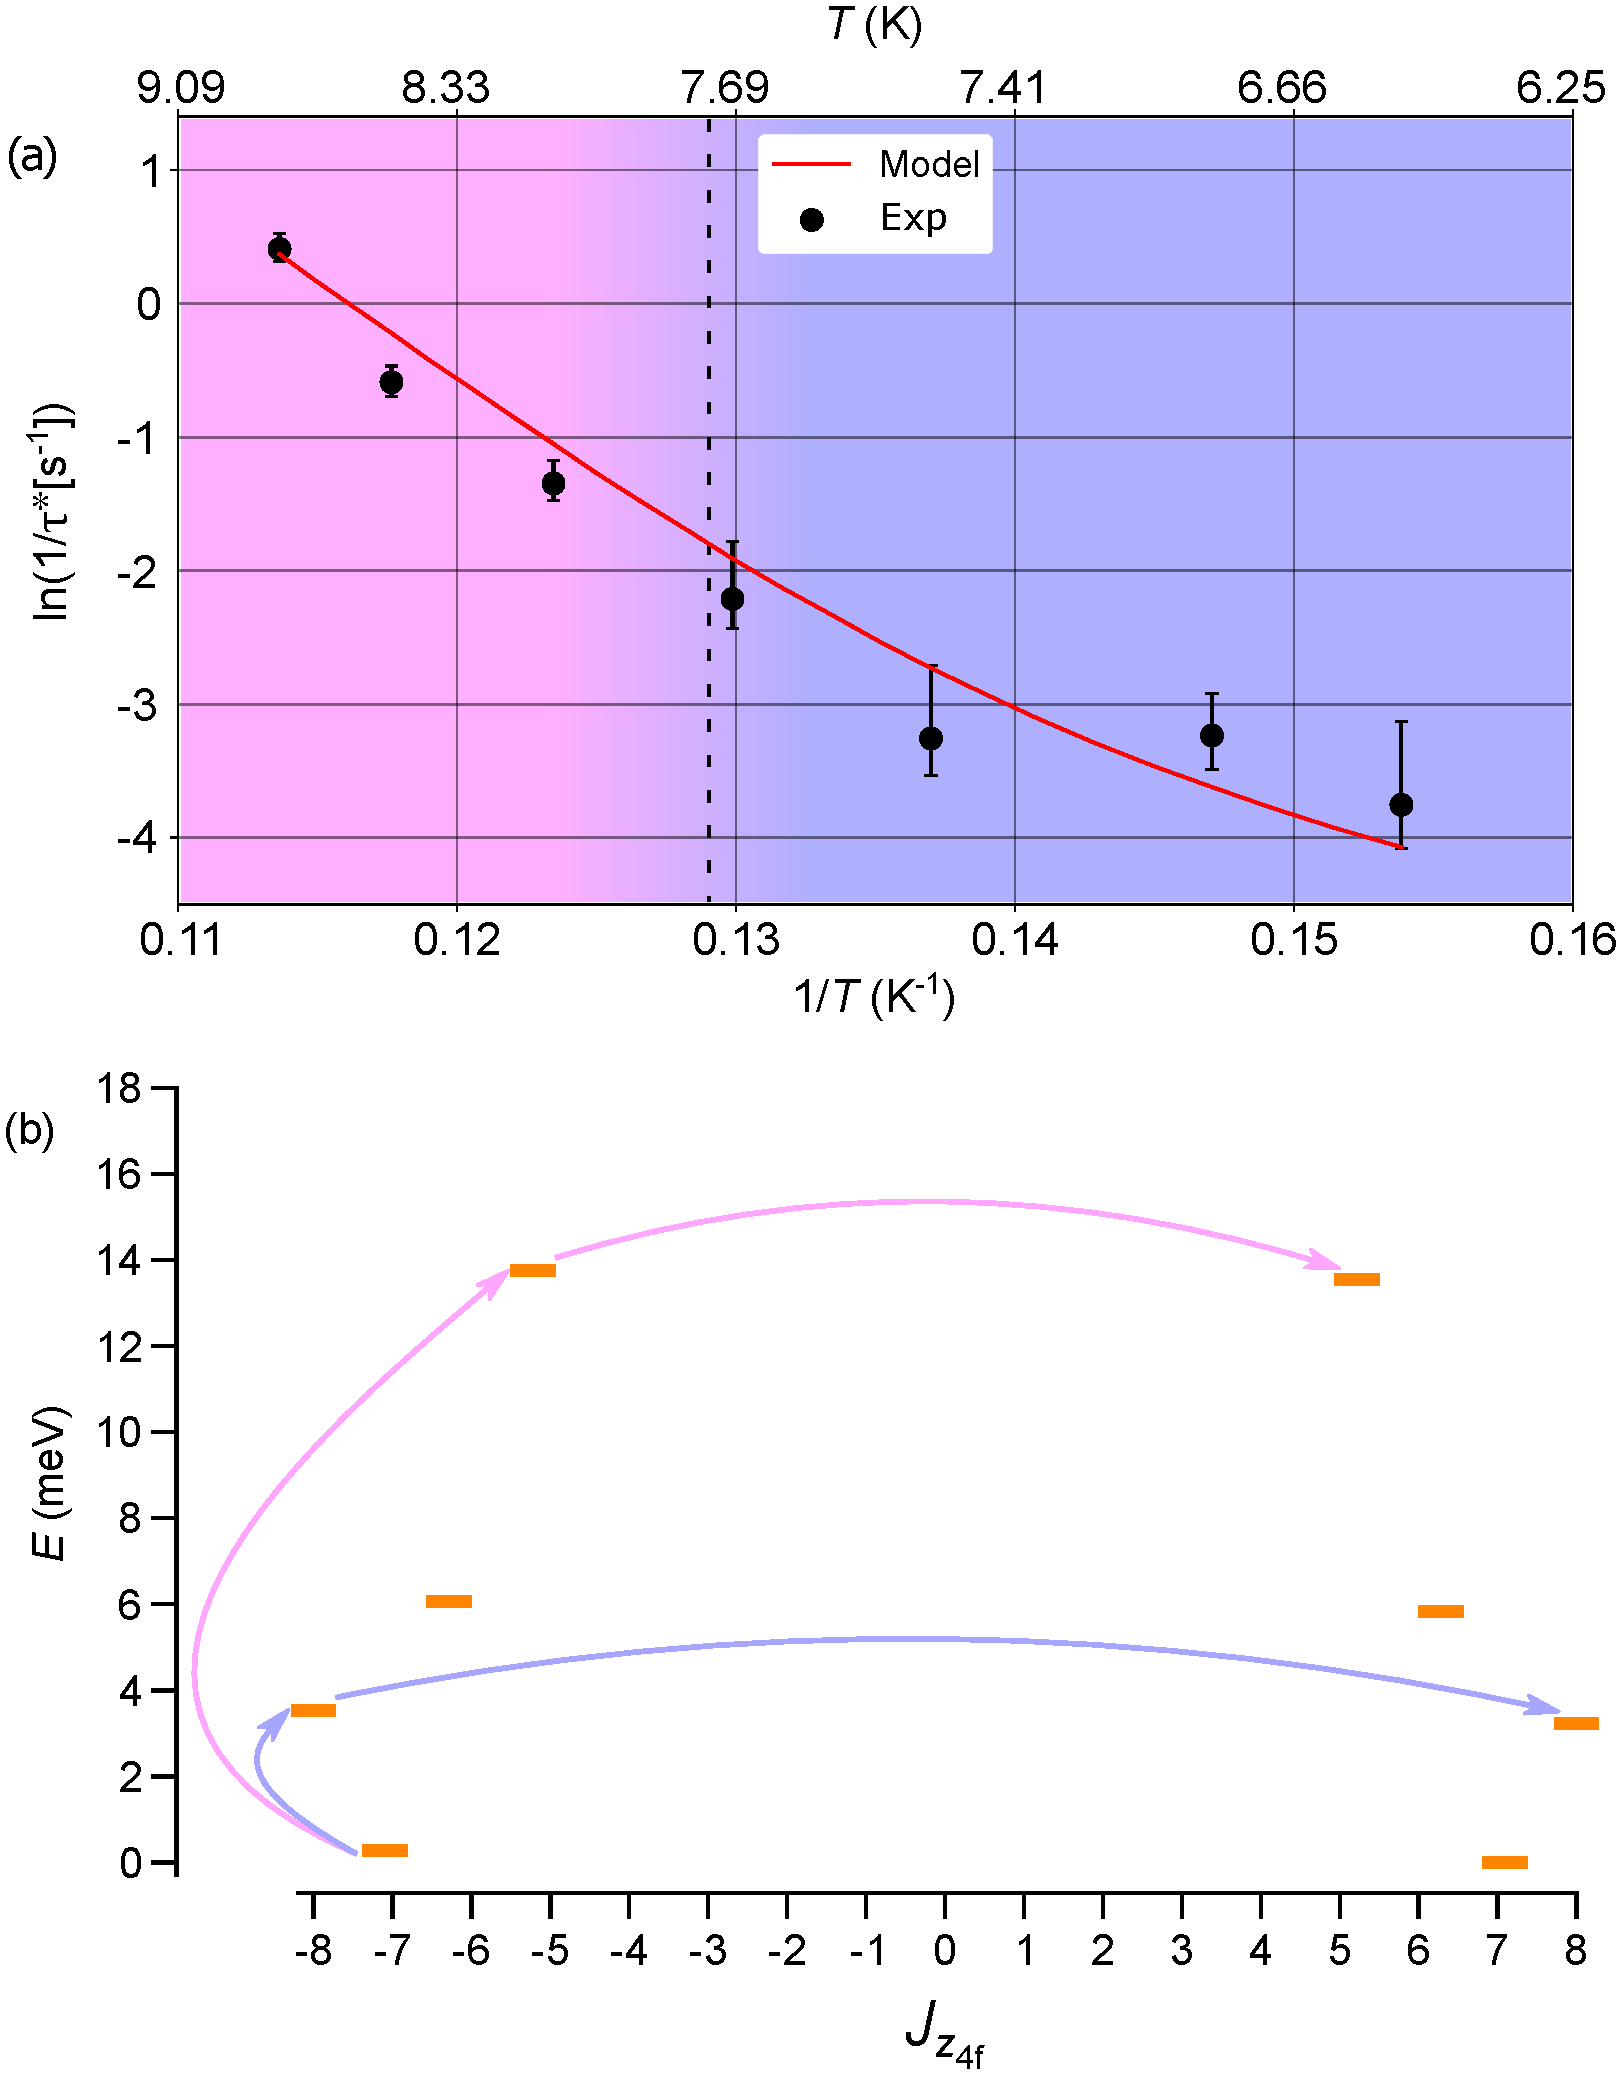
\includegraphics[width=0.5\textwidth]{Fig2_250mT_true.pdf}
\caption{(a) Arrhenious plot of the experimental (black) and model-predicted (red) natural logarithm of the switching frequency (inverse of the lifetime) ($V_{\rm t} = +1$ ~mV, $I_{\rm t} = 10$ ~pA). (b) Level diagram corresponding to the $J_{z}$ states at 250~mT. Each of the $\pm J_{z}$ states are mixed to some degree, such that QTM can occur. The degree of mixing is listed in the Appendix~\ref{app:CF_param}. 
\label{fig:arr+diag}}
\end{figure}

We define the quantity $Tun_{T} = \rho_{T} \nu^{2}_{T}$ where $\rho_{T}$ is the density of states of the tip at the Fermi level and $\nu_{T}$ is a dimensionless factor that is proportional to the tip-adatom hopping integral and therefore scales exponentially with tip-adatom distance. $Tun_{T}$ describes the strength of tip-tip scattering relative to the tip-surface scattering, which is solely responsible for the tunnel current. Additionally, we define an identical quantity for surface-surface scattering: $Tun_{S} = \rho_{S} \nu^{2}_{S}$. Unlike $Tun_{T}$, $Tun_{S}$ is independent of the relative tip-adatom distance and tunnel bias $V_{t}$. In order to fit the experimental data, we require $Tun_{S}$ = 1 and $Tun_{T}$ = 0.02 at 1~mV and 10~pA. The remaining values of $Tun_{T}$ at each experimental data point are listed in the Appendix.\par
We treat the ratio of the spin-flip-assisted to elastic tunnel matrix elements, $\zeta$, as a free parameter. Together with the spin polarization of the tip, $\mathcal{P}_{T} =\frac{\rho_{T \uparrow} - \rho_{T \downarrow}}{\rho_{T \uparrow} + \rho_{T\downarrow}}$ , $\zeta$ determines the magnitude of the elastic magnetoresistant current, which must fit the experimental value. For the telegraph-noise traces used in Figure~\ref{fig:occ}, the magnetoresistive current varies around 10~pA $\pm$ 3~pA. Within the model, we treat $\zeta$ and $\mathcal{P}_{T}$ as constant for all biases with values of 0.2 and 0.7, respectively. With these values, a magnetoresistive current of 7.6~pA is obtained. The expression used to determine the magnetoresistive current is contained in the Supplementary Materials.
Lastly, the quantity $\epsilon_{ph}$ determines proportion of phonons absorbed or de-absorbed between the Dy adatom and graphene per unit time. To explore the effect of phonons on the Dy lifetime, we vary the temperature of the sample while keeping all other tunneling conditions fixed. The results of these measurement are displayed in Figure~\ref{fig:arr+diag}a. $\epsilon_{ph}$ determines the slope of the model points as a function of temperature on the graph. A value of $\epsilon_{ph}$ = $2 \times 10^{-4}$ is used to fit the experimental data.
Figure~\ref{fig:arr+diag}b displays a level diagram of the low energy eigenstates of the model Hamiltonian. The arrows in the figure are the main pathways of magnetization reversal in the Dy adatom. In the low temperature regime, reversal primarily takes place via $\Delta S = \pm 1$  phonon excitation from the $J_{z} = \pm 7$ to the $J_{z} = \pm 8$ state followed by QTM through the anisotropy barrier. At higher temperatures, $\Delta S = \pm 2$ phonon excitation from the $J_{z} = \pm 7$ to the $J_{z} = \pm 5$ state followed by QTM is the dominant pathway. This results in a gradual increase in slope (i.e. the effective energy barrier) in the Arrhenious plot with increasing temperature. 
At energies above 15~mV, the switching frequency of the Dy adatom approaches the acquisition frequency of the STM electronics.
Finally, to further compare the model predictions to the XMCD results, we consider the case when no tip is present. This implies tip-tip scattering and tip-surface scattering rates are nonexistent, and only surface-surface scattering remains. Keeping all other model parameters fixed, and replicating XMCD measurement conditions with $B_{z}$ = 10~mT and $T$ = 2.5~K, we find a lifetime $\tau^*$ = 2527~s. This is consistent with the measured lifetime of around 971~s being a lower limit estimation.

\section{Conclusions}

We use SP-STM to study the spin dynamics of Dy adatoms on graphene/Ir(111) via telegraph-noise traces. A clear spin torque transfer between the tunneling electrons and Dy adatom is present. This results in a strong asymmetry in state occupancy for biases above a few millivolts. We also investigate the temperature dependence on the magnetic lifetime. We are able to model these dynamics by implementing a Kondo-like term for the effect of tunneling electrons and a phonon-scattering term for the effect of phonons in the Hamiltonian. 
\section{Acknowledgements}
\section{Appendix}
\subsection{Crystal Field Parameters}
\label{app:CF_param}
Table I provides the values used for the crystal field parameters $B^{n}_{m}$ in the Hamiltonian. 
\renewcommand{\arraystretch}{2} 
\begin{table}[h!]
\centering
 \begin{tabular}{cccc}
 \hline
 \hline
 $B^{0}_{2}$ ($\mu$eV) & $B^{0}_{4}$ (neV) & $B^{0}_{6}$ (neV) & $B^{6}_{6}$ (neV) 
 \\ [1ex] 
 \hline 
 -136 & 17.5 & 2.45 & -5 \\
 \hline
 \hline
 \end{tabular}
 \caption{CF Parameter Values}
\end{table}
  
\subsection{Model Parameters}
\label{app:STM_param}
Table II provides the values $B_{z}$ and $Tun_{T}$ used for different tunnel biases $V_{t}$. \\

\renewcommand{\arraystretch}{2} 
\begin{table}[H]
\centering
 \begin{tabular}{ccc}
 \hline
 \hline
 $V_{t}$ (mV) & $B_{z}$ (mT) & $Tun_{T}$ 
 \\ [1ex] 
 \hline 
 1.0 & 250 & 0.02 \\
 2.5 & 202.2 & 0.008 \\
 3.5 & 187.7 & 0.0057 \\
 4.5 & 177.8 & 0.0044 \\
 5.5 & 170.4 & 0.0036 \\
 6.5 & 164.5 & 0.0030 \\
 7.5 & 159.7 & 0.0026 \\
 \hline
 \hline
 \end{tabular}
 \caption{Model parameters}
\end{table}


\newpage

\begin{table}
    \begin{tabular}{cccccc}
    \hline
    \hline
    $\ket{M}$ & $j_{4f}$ & $s_{5d}$ & $s_{6s}$ & E (meV) & $\Delta$E (meV)\\
    \hline
    $\ket{\pm 7}$ & $\pm$7.0 & 0 & 0 & 0 & 0     \\
    $\ket{\pm 8}$ & $\pm$8.0 & 0 & 0 & 2.96 & 0    \\
    $\ket{\pm 6}$ & 0 & 0 & 0 & 5.51/5.52 &   1.28 $10^{-2}$   \\
    $\ket{\pm 5}$ & $\pm$5.0 & 0 & 0 & 0 & 0      \\
    \hline
    \hline
    \end{tabular}
\end{table}

\begin{table}
    \begin{tabular}{cccccc}
    \hline
    \hline
    $\ket{M}$ & $j_{4f}$ & $s_{5d}$ & $s_{6s}$ & E (meV) & $\Delta$E (meV)\\
    \hline
    $\ket{\pm 7}$ & $\pm$7.1 & $\pm$0.5 & $\pm$0.5 & 0 & 0     \\
    $\ket{\pm 8}$ & 0 & 0 & 0 & 3.25 & 2.4 $10^{-5}$    \\
    $\ket{\pm 6}$ & $\pm$6.3 & $\pm$0.4 & $\pm$0.4 & 5.82 &   0   \\
    $\ket{\pm 5}$ & 0 & 0 & 0 & 13.48/13.54 & 6.0 $10^{-2}$       \\ 
    \hline
    \hline
    \end{tabular}
\end{table}

\begin{table}
    \begin{tabular}{cccccc}
    \hline
    \hline
    $\ket{M}$ & $j_{4f}$ & $s_{5d}$ & $s_{6s}$ & E (meV) & $\Delta$E (meV)\\
    \hline
    $\ket{\pm 7}$ & $\pm$7.0 & 0 & 0 & 0 & 0     \\
    $\ket{\pm 8}$ & $\pm$8.0 & 0 & 0 & 3.0 & 0    \\
    $\ket{\pm 6}$ & 0 & 0 & 0 & 5.5 &   1.3 $10^{-2}$   \\
    $\ket{\pm 5}$ & $\pm$5.0 & 0 & 0 & 0 & 0      \\
    \hline
    \hline
    \end{tabular}
\end{table}

\begin{table}
    \begin{tabular}{cccccc}
    \hline
    \hline
    $\ket{M}$ & $j_{4f}$ & $s_{5d}$ & $s_{6s}$ & E (meV) & $\Delta$E (meV)\\
    \hline
    $\ket{\pm 7}$ & $\pm$7.1 & $\pm$0.5 & $\pm$0.5 & 0 & 0     \\
    $\ket{\pm 8}$ & 0 & 0 & 0 & 3.3 & 2.4 $10^{-5}$    \\
    $\ket{\pm 6}$ & $\pm$6.3 & $\pm$0.4 & $\pm$0.4 & 5.8 &   0   \\
    $\ket{\pm 5}$ & 0 & 0 & 0 & 13.5 & 6.0 $10^{-2}$       \\ 
    \hline
    \hline
    \end{tabular}
\end{table}



\bibliographystyle{unsrt}
\bibliography{bib.bib}

\end{document}

